\documentclass[aspectratio=169,11pt]{beamer}

% Theme and colors
\usetheme{Madrid}
\usecolortheme{whale}
\setbeamertemplate{navigation symbols}{}
\setbeamertemplate{footline}[frame number]

% Packages
\usepackage[utf8]{inputenc}
\usepackage{graphicx}
\usepackage{booktabs}
\usepackage{amsmath}
\usepackage{tikz}
\usepackage{pgfplots}
\pgfplotsset{compat=1.18}

% Custom colors
\definecolor{UBblue}{RGB}{0,82,147}
\definecolor{UBgold}{RGB}{255,184,28}
\setbeamercolor{structure}{fg=UBblue}
\setbeamercolor{block title}{bg=UBblue,fg=white}

% Title info
\title[Solar Forecasting]{Multi-Site Solar Irradiance Forecasting}
\subtitle{A Comparative Study of SARIMA, GRU, and Graph Neural Networks}
\author[Dalmau \& Perry]{Ferran Dalmau Codina \and Christofer Perry}
\institute[UB]{Universitat de Barcelona\\Master's in Data Science}
\date{June 2026}

\begin{document}

% ============================================================================
% TITLE SLIDE
% ============================================================================
\begin{frame}
\titlepage
\end{frame}

% ============================================================================
% OUTLINE
% ============================================================================
\begin{frame}{Outline}
\tableofcontents
\end{frame}

% ============================================================================
% SECTION 1: INTRODUCTION
% ============================================================================
\section{Introduction}

\begin{frame}{Motivation}
\begin{columns}
\column{0.6\textwidth}
\textbf{Why solar forecasting matters:}
\begin{itemize}
    \item Grid integration and stability
    \item Energy market trading (day-ahead, intra-day)
    \item Battery storage optimization
    \item Demand-side management
\end{itemize}

\vspace{0.5cm}
\textbf{The challenge:}
\begin{itemize}
    \item Clearsky irradiance is deterministic
    \item \alert{Clouds} are the source of uncertainty
    \item Clouds move spatially $\rightarrow$ multi-site approach
\end{itemize}

\column{0.4\textwidth}
\centering
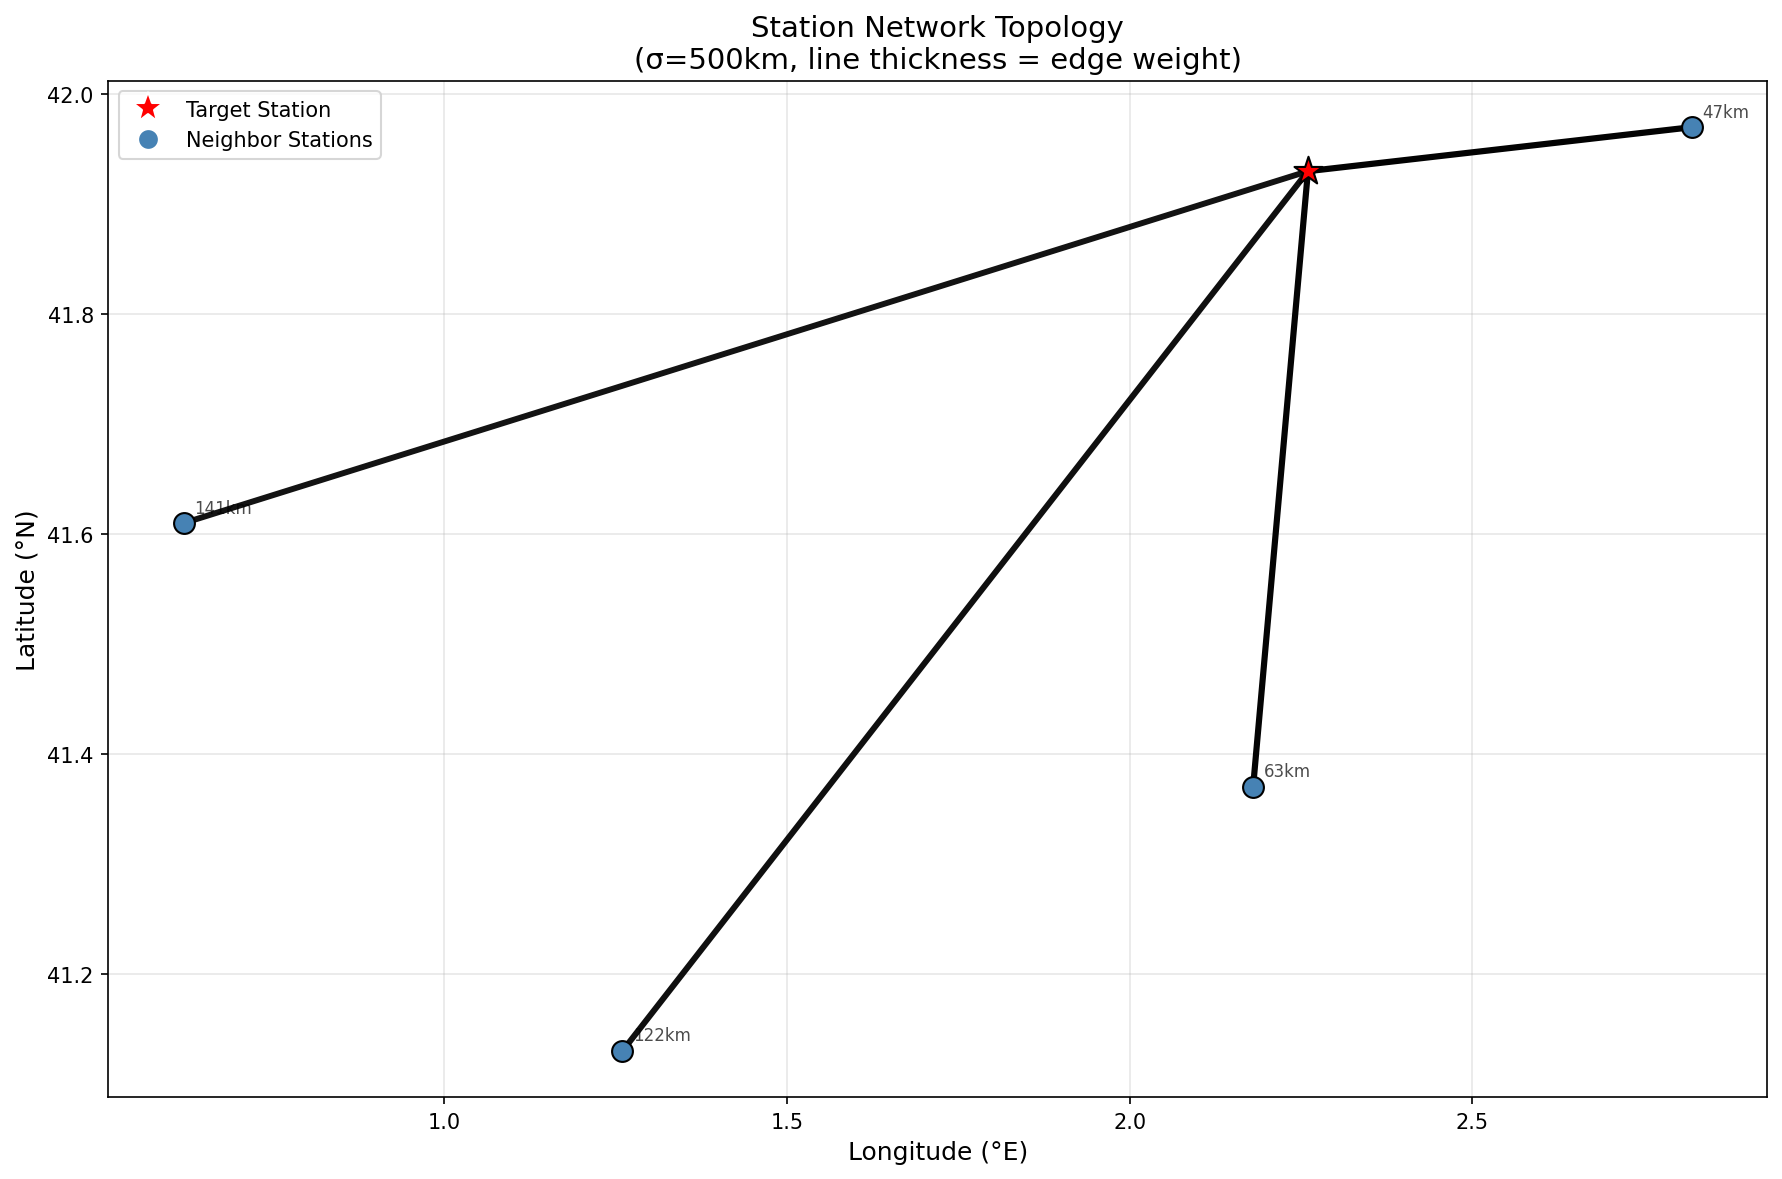
\includegraphics[width=\textwidth]{../figures/station_network_topology.png}
\end{columns}
\end{frame}

\begin{frame}{Research Objectives}
\begin{enumerate}
    \item \textbf{Compare} three forecasting methodologies:
    \begin{itemize}
        \item SARIMA (classical time series)
        \item SolarGRU (deep learning)
        \item SolarGNN (graph neural network)
    \end{itemize}
    
    \vspace{0.3cm}
    \item \textbf{Evaluate} at three operationally relevant horizons:
    \begin{itemize}
        \item 1h (intra-hour scheduling)
        \item 6h (intra-day trading)
        \item 24h (day-ahead planning)
    \end{itemize}
    
    \vspace{0.3cm}
    \item \textbf{Demonstrate} the value of multi-site data
    
    \vspace{0.3cm}
    \item \textbf{Analyze} robustness under sensor failures
\end{enumerate}
\end{frame}

% ============================================================================
% SECTION 2: DATA
% ============================================================================
\section{Data \& Preprocessing}

\begin{frame}{Data Source: NREL NSRDB}
\begin{columns}
\column{0.5\textwidth}
\textbf{National Solar Radiation Database:}
\begin{itemize}
    \item 15-minute resolution
    \item 2020--2023 (3 years)
    \item $\sim$105,000 timesteps
\end{itemize}

\vspace{0.3cm}
\textbf{Station configuration:}
\begin{itemize}
    \item Target: Spain Central (41.93°N)
    \item Neighbor: Atlantic (upstream)
    \item Distance: $\sim$3,500 km
\end{itemize}

\column{0.5\textwidth}
\textbf{Variables:}
\begin{itemize}
    \item GHI, DNI, DHI
    \item Clearsky GHI
    \item Cloud Type (0--12)
    \item Temperature, Humidity
    \item Wind Speed/Direction
    \item Pressure, Dew Point
\end{itemize}
\end{columns}
\end{frame}

\begin{frame}{Clearsky Index Transformation}
\begin{block}{Key Innovation}
Predict $kt$ instead of raw GHI:
\[
kt = \frac{\text{GHI}}{\text{Clearsky GHI} + \epsilon}
\]
\end{block}

\vspace{0.3cm}
\textbf{Advantages:}
\begin{itemize}
    \item Removes deterministic astronomical variation
    \item Bounded range: $kt \in [0, \sim1.5]$
    \item Interpretable: $kt \approx 1$ = clear, $kt < 0.5$ = cloudy
    \item Easy reconstruction: $\hat{\text{GHI}} = \hat{kt} \times \text{Clearsky GHI}$
\end{itemize}
\end{frame}

% ============================================================================
% SECTION 3: METHODOLOGY
% ============================================================================
\section{Methodology}

\begin{frame}{Model A: SARIMA}
\begin{columns}
\column{0.5\textwidth}
\textbf{Specification:}
\[
\text{SARIMA}(1,0,1)(1,1,1)_{24}
\]

\begin{itemize}
    \item Hourly aggregation ($s = 24$)
    \item Direct forecasting per horizon
    \item 3 separate models fitted
\end{itemize}

\column{0.5\textwidth}
\textbf{Limitations:}
\begin{itemize}
    \item Univariate (target only)
    \item Linear assumptions
    \item Loses sub-hourly dynamics
\end{itemize}
\end{columns}
\end{frame}

\begin{frame}{Model B: SolarGRU}
\centering
\begin{tikzpicture}[scale=0.8, every node/.style={scale=0.8}]
    % Target GRU
    \node[draw, rectangle, minimum width=2.5cm, minimum height=1cm, fill=blue!20] (tgru) at (0,2) {GRU (64, 2 layers)};
    \node[above=0.3cm of tgru] {Target: 14 features};
    
    % Neighbor GRU
    \node[draw, rectangle, minimum width=2.5cm, minimum height=1cm, fill=green!20] (ngru) at (5,2) {GRU (32, 1 layer)};
    \node[above=0.3cm of ngru] {Neighbor: 6 features};
    
    % Concat
    \node[draw, rectangle, minimum width=4cm, minimum height=0.8cm, fill=orange!20] (concat) at (2.5,0) {Concat (96) + LayerNorm};
    
    % Output
    \node[draw, rectangle, minimum width=3cm, minimum height=0.8cm, fill=red!20] (out) at (2.5,-1.5) {Linear $\rightarrow$ GELU $\rightarrow$ Sigmoid};
    
    % Predictions
    \node[below=0.3cm of out] {$\hat{kt}$ at 1h, 6h, 24h};
    
    % Arrows
    \draw[->, thick] (tgru) -- (concat);
    \draw[->, thick] (ngru) -- (concat);
    \draw[->, thick] (concat) -- (out);
\end{tikzpicture}

\vspace{0.5cm}
\textbf{Key features:} Asymmetric encoders, multi-output head, 24h lookback
\end{frame}

\begin{frame}{Model C: SolarGNN}
\begin{columns}
\column{0.5\textwidth}
\textbf{Graph Construction:}
\[
w_{ij} = \exp\left(-\frac{d_{ij}^2}{\sigma^2}\right)
\]

\begin{itemize}
    \item Nodes = stations
    \item Edges = Gaussian kernel weights
    \item $\sigma = 100$ km decay
\end{itemize}

\column{0.5\textwidth}
\textbf{Architecture:}
\begin{enumerate}
    \item GCN layers (spatial aggregation)
    \item Extract target node features
    \item GRU (temporal encoding)
    \item Multi-horizon prediction head
\end{enumerate}
\end{columns}

\vspace{0.5cm}
\centering
\alert{Advantage:} Explicitly encodes geographic relationships
\end{frame}

% ============================================================================
% SECTION 4: RESULTS
% ============================================================================
\section{Results}

\begin{frame}{Model Performance Comparison}
\centering
\begin{tabular}{llccc}
\toprule
\textbf{Horizon} & \textbf{Model} & \textbf{RMSE} & \textbf{Skill} & \textbf{$R^2$} \\
\midrule
\multirow{3}{*}{1h} 
& SARIMA & 0.212 & 0.057 & 0.729 \\
& \textbf{SolarGRU} & \textbf{0.162} & \textbf{0.436} & \textbf{0.855} \\
& SolarGNN & 0.177 & 0.384 & 0.827 \\
\midrule
\multirow{3}{*}{6h}
& SARIMA & 0.210 & 0.621 & 0.735 \\
& \textbf{SolarGRU} & \textbf{0.207} & \textbf{0.644} & \textbf{0.763} \\
& SolarGNN & 0.216 & 0.628 & 0.742 \\
\midrule
\multirow{3}{*}{24h}
& SARIMA & 0.217 & 0.186 & 0.717 \\
& \textbf{SolarGRU} & 0.225 & \textbf{0.228} & \textbf{0.720} \\
& SolarGNN & 0.230 & 0.210 & 0.707 \\
\bottomrule
\end{tabular}

\vspace{0.3cm}
\textbf{Key finding:} SolarGRU outperforms at all horizons
\end{frame}

\begin{frame}{Skill Score Comparison}
\centering
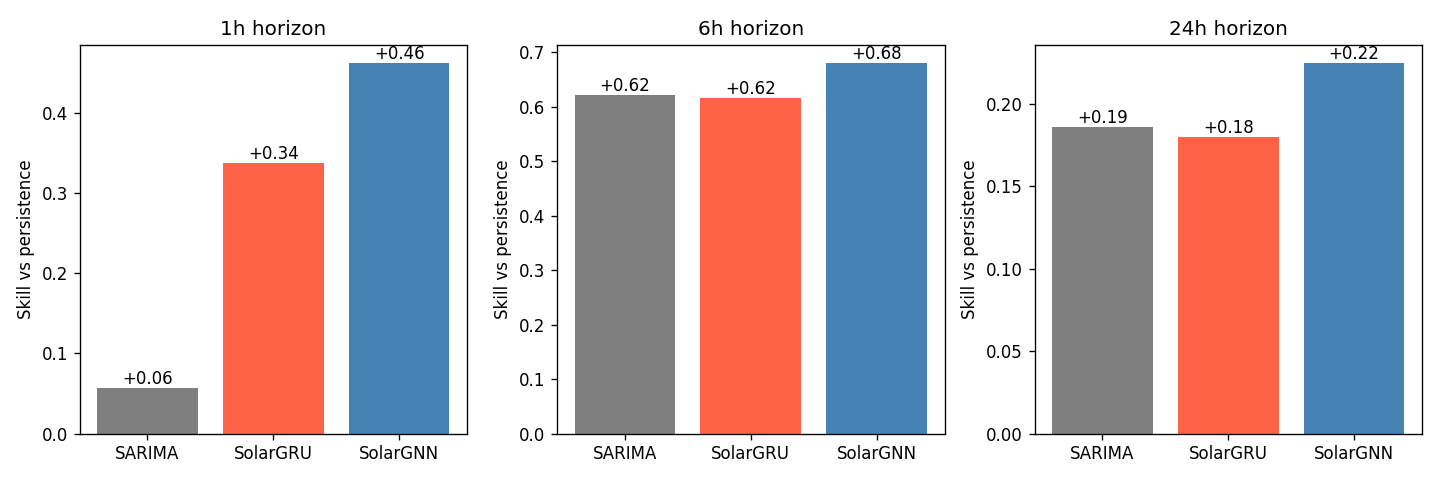
\includegraphics[width=0.9\textwidth]{../figures/skill_scores.png}
\end{frame}

\begin{frame}{Time Series Visualization}
\centering
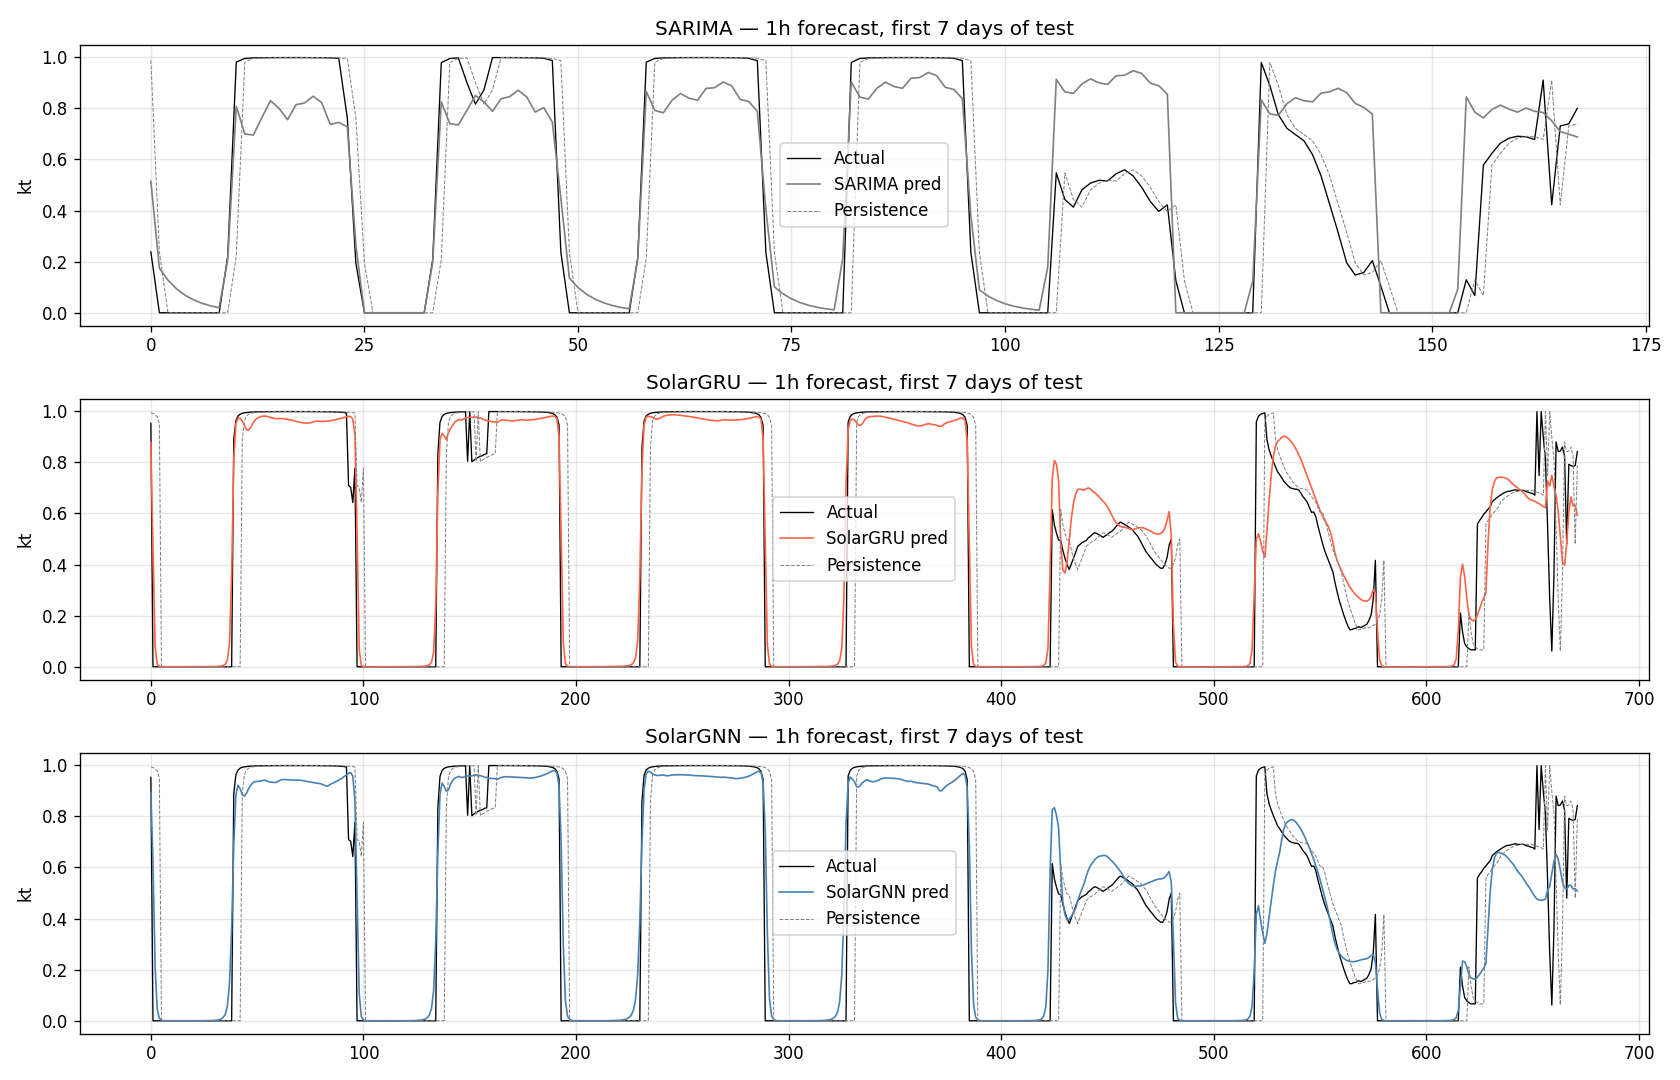
\includegraphics[width=0.95\textwidth]{../figures/timeseries_first_week.png}
\end{frame}

% ============================================================================
% SECTION 5: ROBUSTNESS ANALYSIS (NEW)
% ============================================================================
\section{Robustness Analysis}

\begin{frame}{Multi-Site vs Single-Station}
\begin{block}{Key Question}
Does incorporating data from neighboring stations improve forecasts?
\end{block}

\vspace{0.5cm}
\centering
\begin{tabular}{lccc}
\toprule
\textbf{Configuration} & \textbf{1h Skill} & \textbf{6h Skill} & \textbf{24h Skill} \\
\midrule
\textbf{Multi-Site} (with neighbor) & 0.163 & \textbf{0.493} & \textbf{0.646} \\
Single-Station (target only) & 0.155 & 0.468 & 0.626 \\
\midrule
\textbf{Improvement} & +5.2\% & \textbf{+5.3\%} & +3.2\% \\
\bottomrule
\end{tabular}

\vspace{0.5cm}
\alert{Yes!} Multi-site consistently outperforms single-station
\end{frame}

\begin{frame}{Station Dropout Scenarios}
\centering
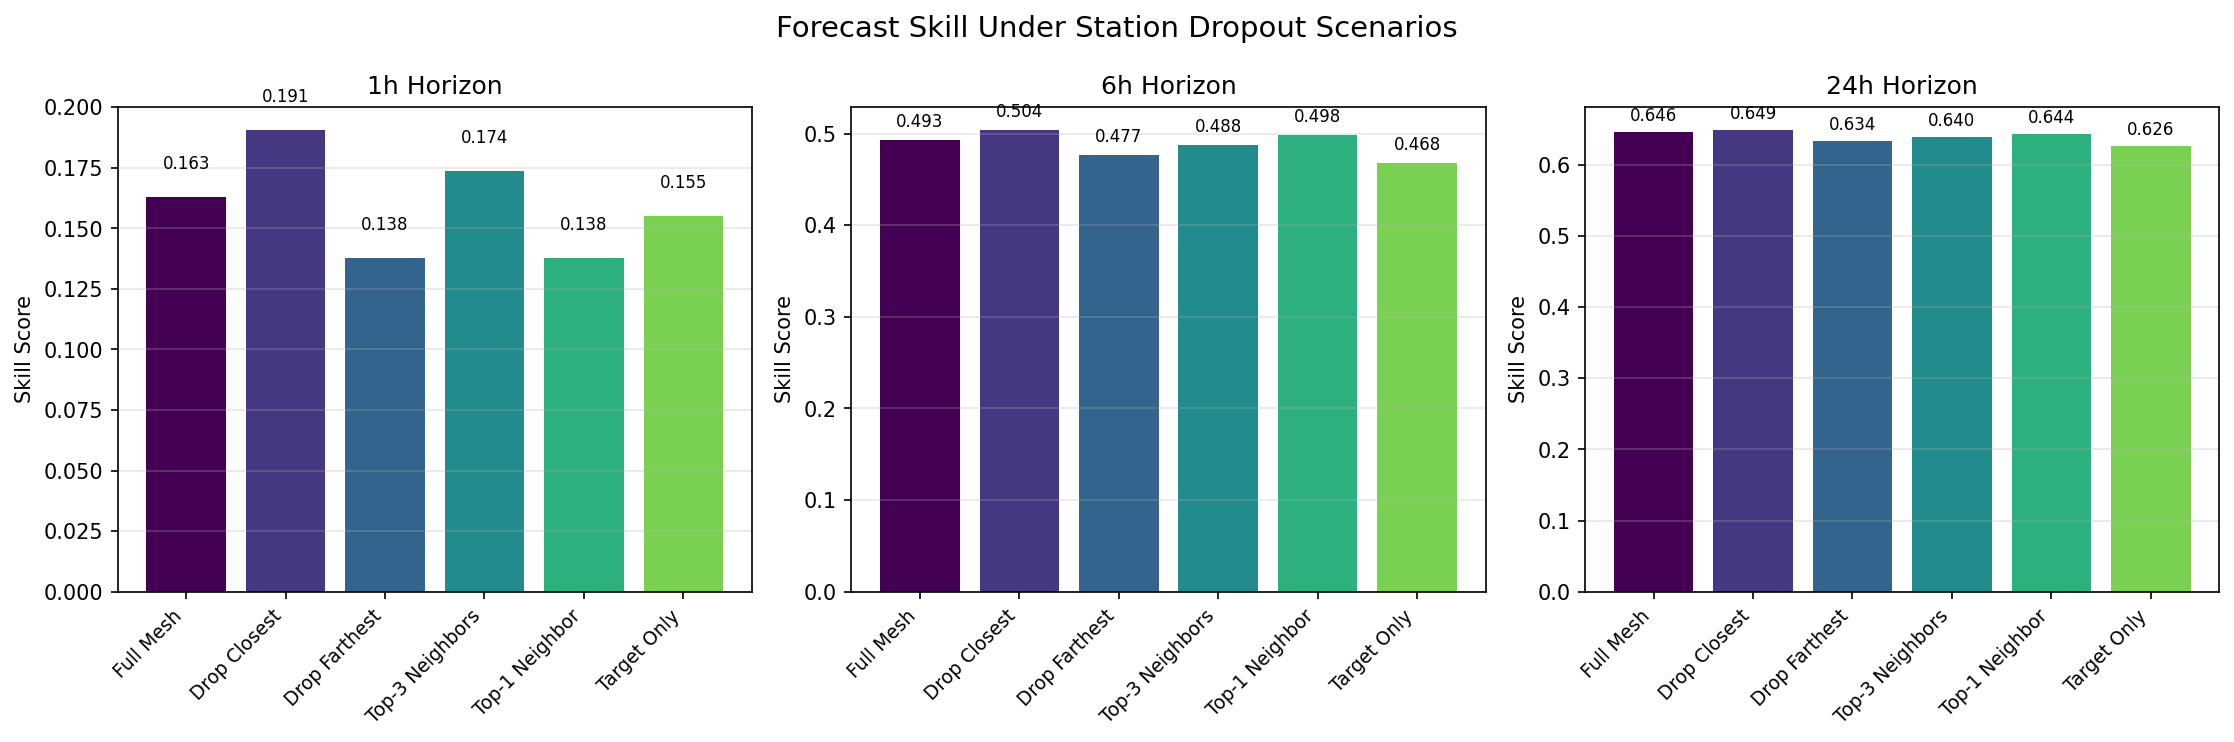
\includegraphics[width=0.85\textwidth]{../figures/robustness_skill_comparison.png}

\vspace{0.3cm}
\textbf{Finding:} System maintains $>$95\% performance even when neighbor fails
\end{frame}

\begin{frame}{Performance Degradation Heatmap}
\centering
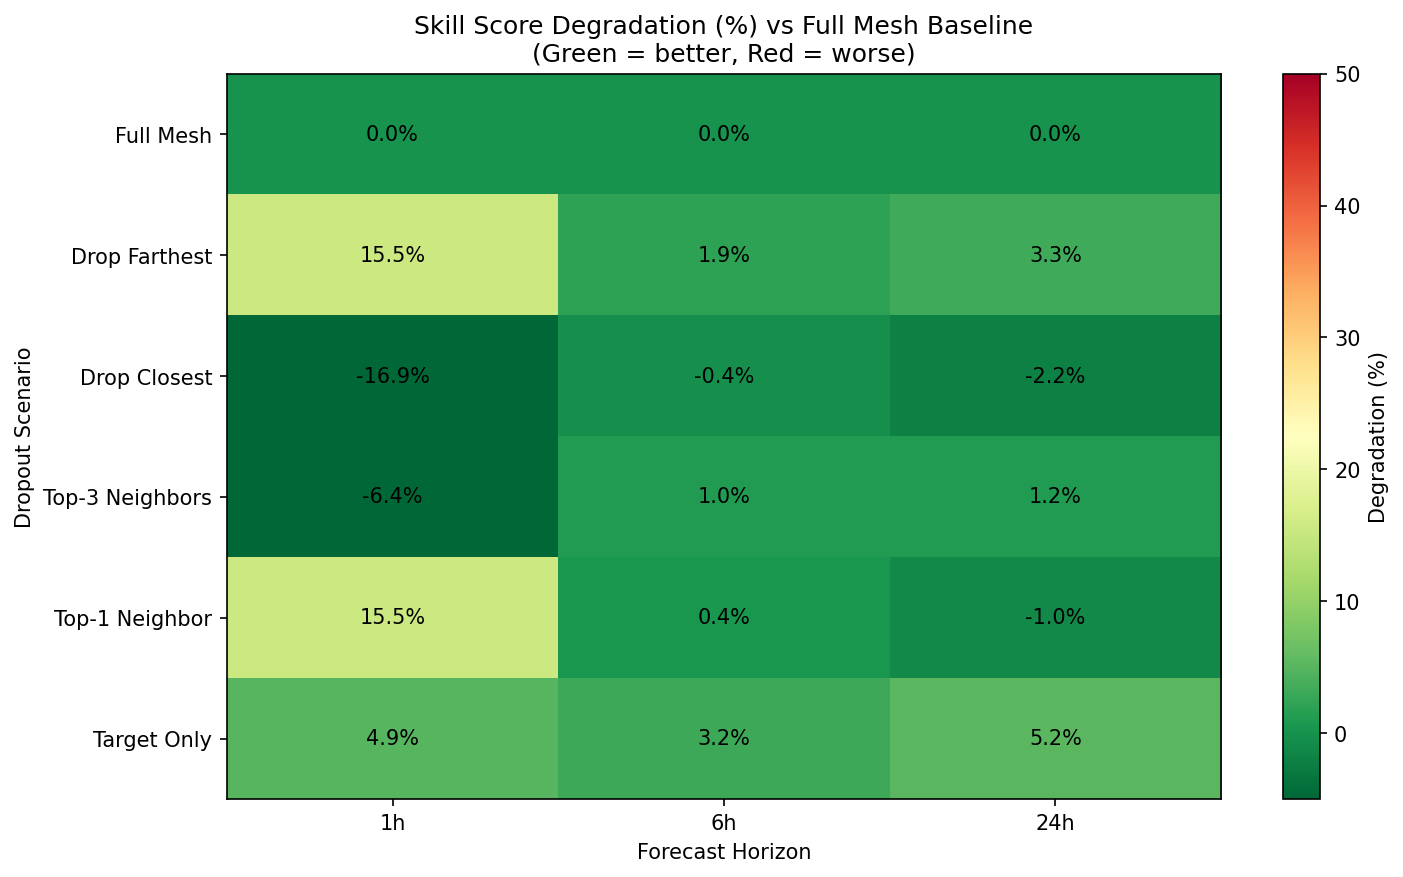
\includegraphics[width=0.75\textwidth]{../figures/robustness_degradation_heatmap.png}

\vspace{0.3cm}
\textbf{Graceful degradation:} Max 5\% loss at 6h, <3.5\% at 24h
\end{frame}

% ============================================================================
% SECTION 6: CASE STUDY (NEW)
% ============================================================================
\section{Case Study: Spatiotemporal Advantage}

\begin{frame}{Per-Sample Analysis}
\centering
\begin{tabular}{lcccc}
\toprule
\textbf{Horizon} & \textbf{Multi-Site MAE} & \textbf{Single-Stn MAE} & \textbf{Improvement} & \textbf{Multi-Site Wins} \\
\midrule
1h & 0.128 & 0.123 & $-4.3\%$ & 43.7\% \\
6h & 0.180 & 0.185 & $+3.0\%$ & 56.0\% \\
24h & 0.228 & 0.257 & $\mathbf{+11.4\%}$ & \textbf{62.0\%} \\
\bottomrule
\end{tabular}

\vspace{0.5cm}
\begin{alertblock}{Key Insight}
Multi-site advantage \textbf{increases with horizon}:
\begin{itemize}
    \item 1h: No clear advantage (44\% win rate)
    \item 24h: Strong advantage (62\% win rate, 11.4\% MAE improvement)
\end{itemize}
\end{alertblock}
\end{frame}

\begin{frame}{Physical Interpretation}
\begin{columns}
\column{0.5\textwidth}
\textbf{Why horizon matters:}

Weather systems propagate from Atlantic $\rightarrow$ Spain

\vspace{0.3cm}
\begin{itemize}
    \item \textbf{1h horizon:} Cloud patterns at upstream station haven't arrived yet
    \item \textbf{24h horizon:} Upstream station ``sees'' fronts 12--24h before arrival
\end{itemize}

\column{0.5\textwidth}
\centering
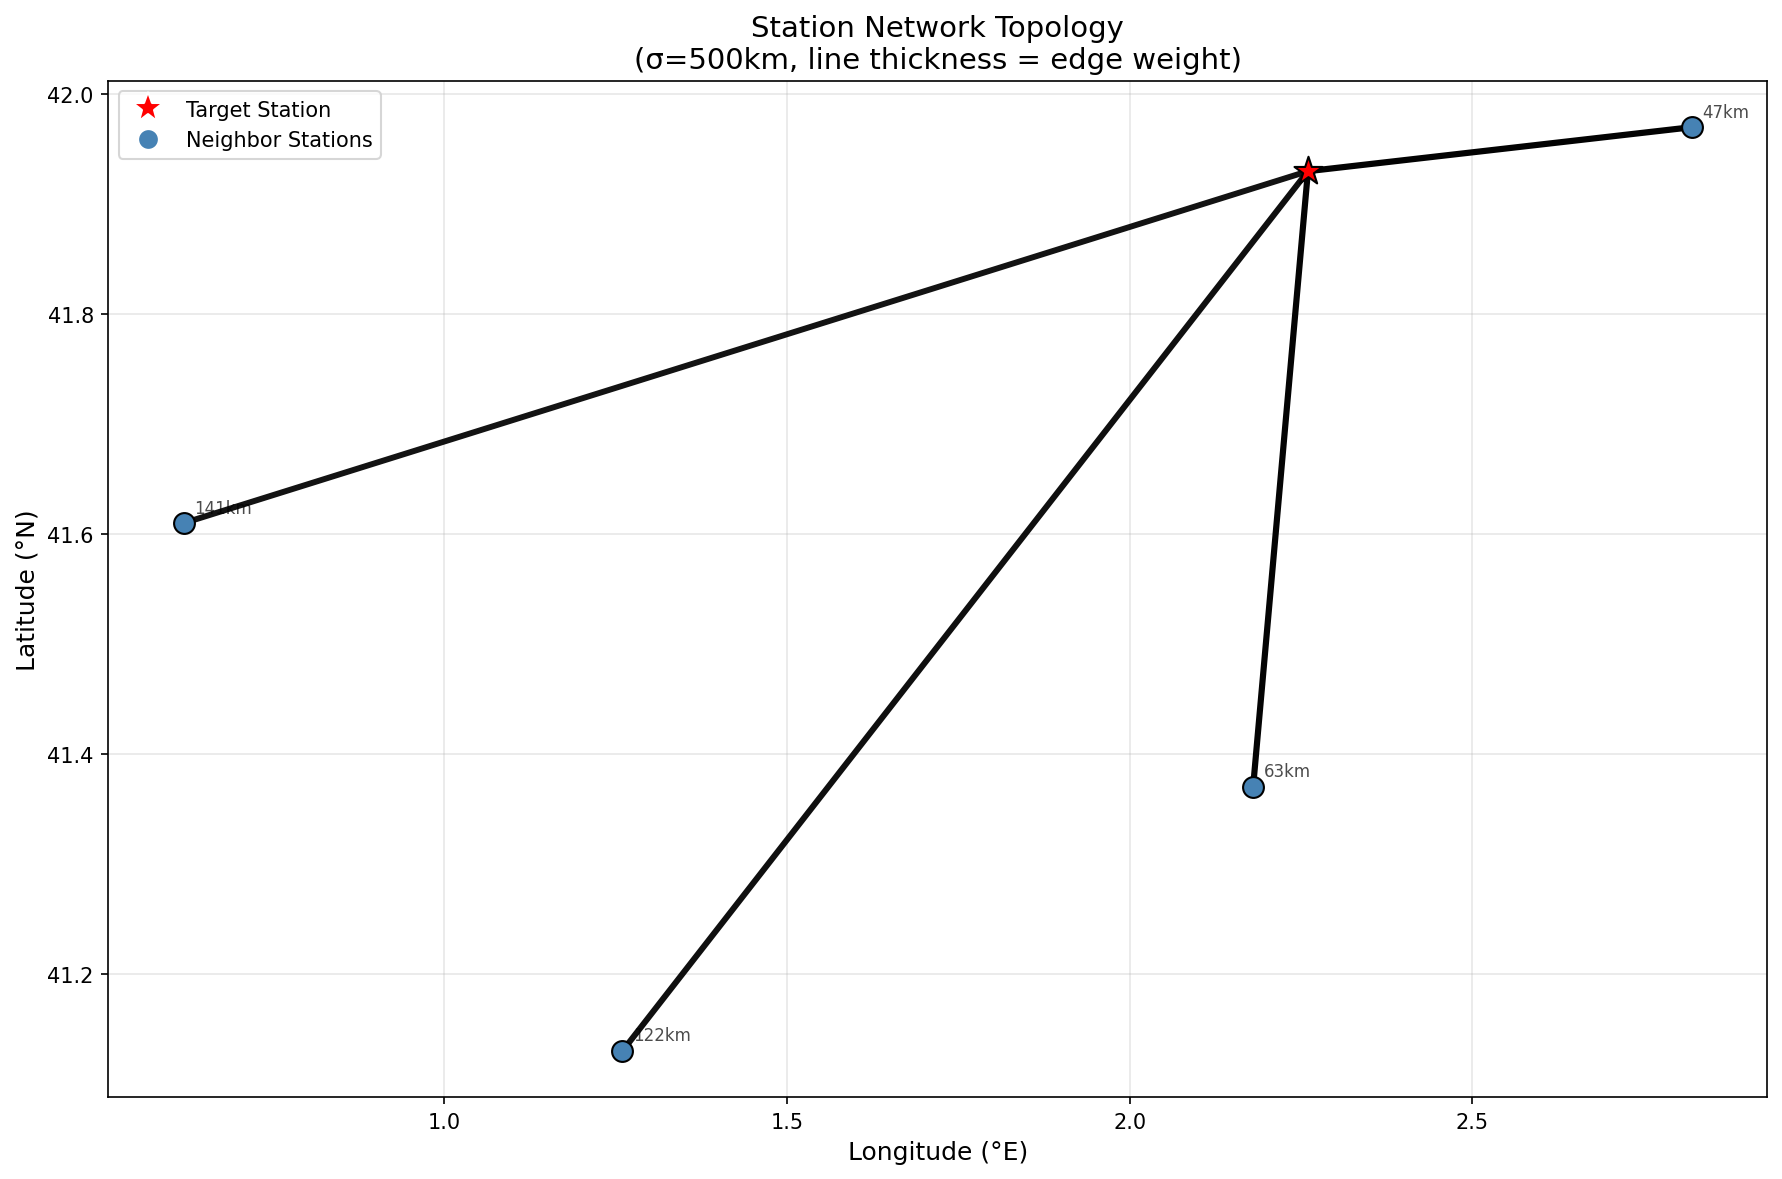
\includegraphics[width=\textwidth]{../figures/station_network_topology.png}
\end{columns}

\vspace{0.5cm}
\centering
\alert{Multi-site provides early warning for incoming cloud fronts}
\end{frame}

\begin{frame}{Cloud Front Detection Case Study}
\centering
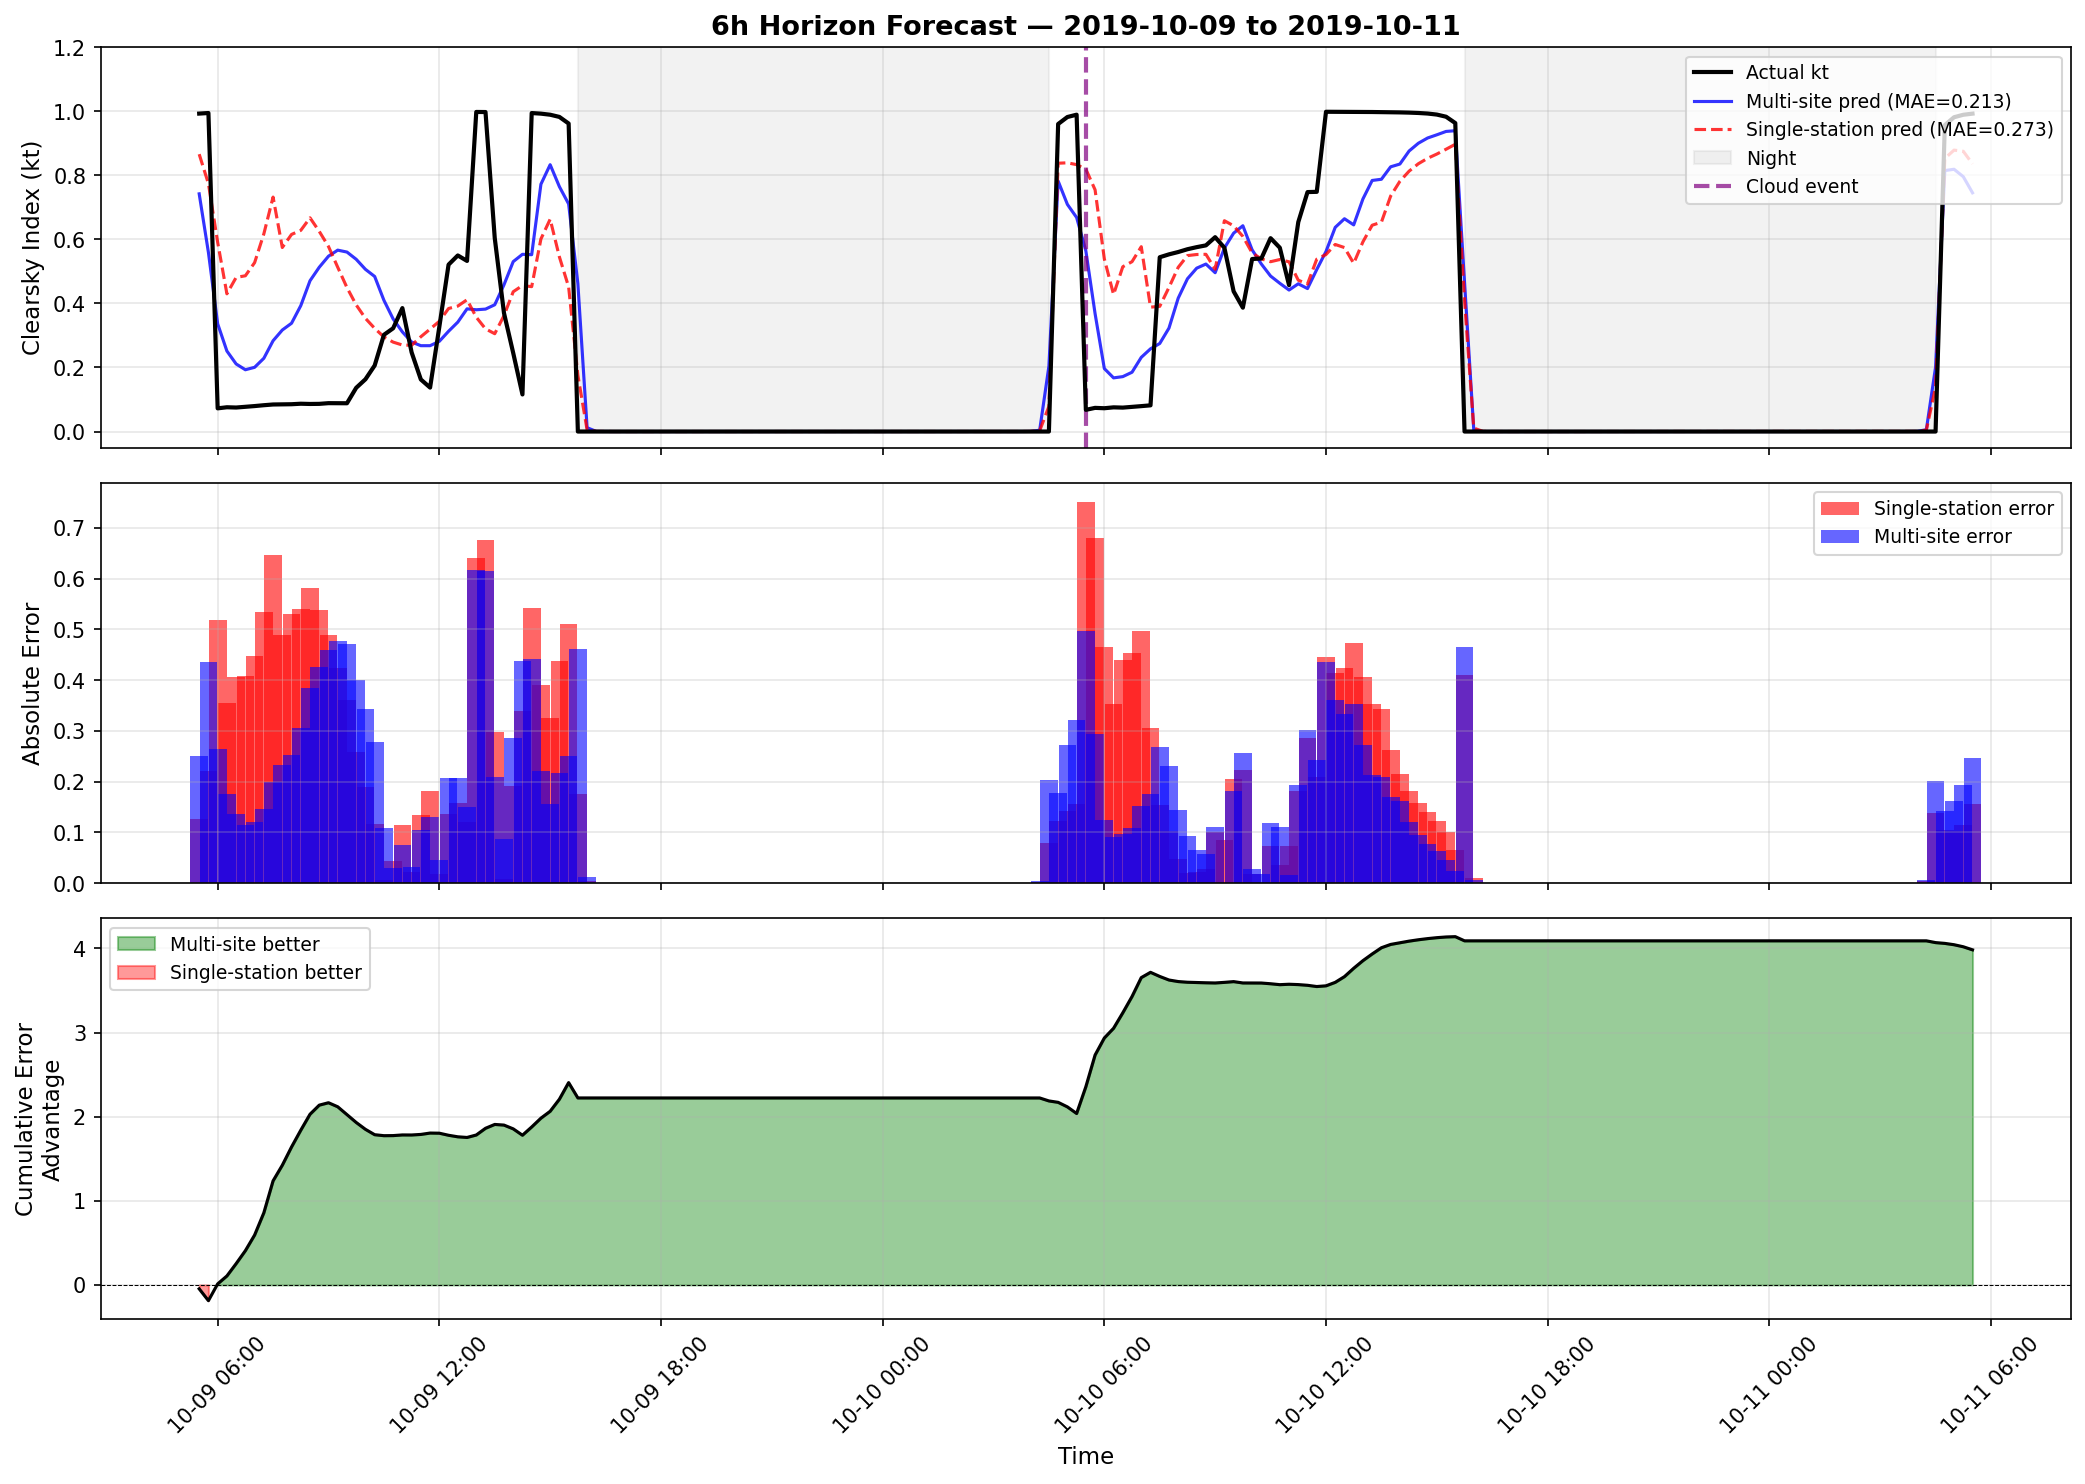
\includegraphics[width=0.9\textwidth]{../figures/case_study_cloud_event.png}
\end{frame}

\begin{frame}{Error Scatter Comparison}
\centering
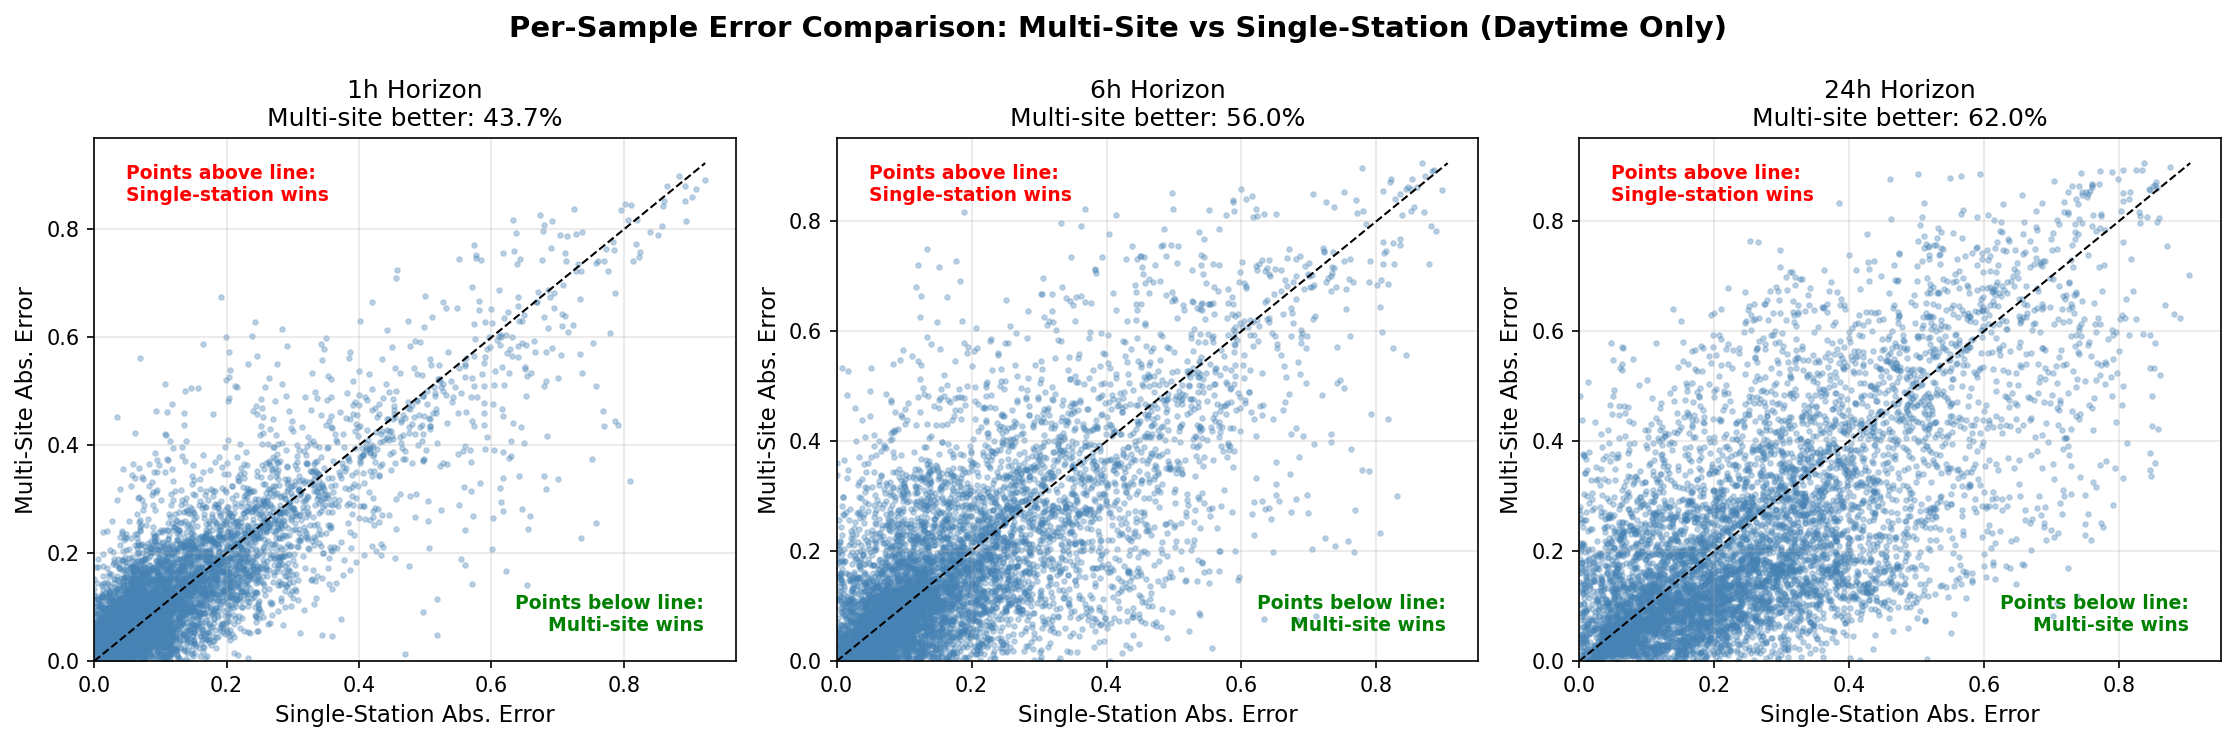
\includegraphics[width=0.95\textwidth]{../figures/error_scatter_comparison.png}

\vspace{0.3cm}
Points below diagonal = multi-site wins
\end{frame}

% ============================================================================
% SECTION 7: CONCLUSIONS
% ============================================================================
\section{Conclusions}

\begin{frame}{Key Takeaways}
\begin{enumerate}
    \item \textbf{Neural approaches outperform SARIMA} at all horizons (30--60\% skill improvement)
    
    \vspace{0.3cm}
    \item \textbf{Clearsky index transformation} effectively removes astronomical variability
    
    \vspace{0.3cm}
    \item \textbf{Multi-site advantage increases with horizon}:
    \begin{itemize}
        \item 62\% win rate at 24h (vs 44\% at 1h)
        \item 11.4\% MAE improvement at day-ahead
    \end{itemize}
    
    \vspace{0.3cm}
    \item \textbf{Graceful degradation:} System retains $>$95\% performance under sensor failures
    
    \vspace{0.3cm}
    \item \textbf{6h horizon} is the ``sweet spot'' for learned models
\end{enumerate}
\end{frame}

\begin{frame}{Future Work}
\begin{itemize}
    \item Expand station network (5--10 stations across Iberian Peninsula)
    \item Incorporate NWP forecasts as exogenous inputs
    \item Probabilistic forecasting (prediction intervals)
    \item Attention mechanisms (Transformers)
    \item Real-time operational deployment
\end{itemize}

\vspace{1cm}
\centering
\Large\textbf{Thank you!}

\vspace{0.5cm}
\normalsize
Questions?
\end{frame}

\end{document}
